%---------------------------------------------------------------------------------------

\chapter[Resultados]{Resultados}\label{ch:resultados}

%---------------------------------------------------------------------------------------

% Lista de abreviaturas e de siglas
\criarsigla{EQM}{Erro quadrático médio}

%---------------------------------------------------------------------------------------

% Lista de simbolos

%---------------------------------------------------------------------------------------

A campanha de ensaios conduzida com o miniaplicativo de Lattice Boltzmann para escoamentos compressíveis contemplou quatro dimensões de avaliação: a validação física do escoamento, a sensibilidade paramétrica do método, a escalabilidade em unidades centrais de processamento (CPUs) e a comparação de desempenho e de complexidade entre as tecnologias de paralelização em arquiteturas heterogêneas, incluindo unidades de processamento gráfico (GPUs).
Todos os ensaios partiram da mesma configuração de referência e foram executados na máquina descrita no Capítulo~\ref{ch:metodologia}, de modo que as diferenças observadas possam ser atribuídas exclusivamente ao fator variado em cada caso.

A validação precede as medições de desempenho por uma razão metodológica: nenhuma implementação foi admitida na campanha de medições antes de reproduzir os campos macroscópicos da versão sequencial de referência dentro da tolerância estabelecida na Seção~\ref{sec:delineamento-da-pesquisa}.
Os resultados de desempenho relatados adiante referem-se, portanto, a versões numericamente equivalentes entre si, condição sem a qual a comparação entre tecnologias perderia sentido.

%---------------------------------------------------------------------------------------

\section{Validação com o Tubo de Choque de Sod}\label{sec:validacao-tubo-de-choque-de-sod}

O protocolo experimental para a validação física consistiu na execução do miniaplicativo utilizando a configuração de referência detalhada no arquivo \texttt{config.yaml}, a qual define um domínio unitário com \(N_x = 50000\) nós na direção longitudinal e \(N_y = N_x/100\) nós na direção transversal.
As condições iniciais e as propriedades do fluido são as reunidas na \autoref{tab:parametros-simulacao} do Capítulo~\ref{ch:metodologia}, a saber, \((\rho_L;\ p_L) = (1{,}0;\ 1{,}0)\) e \((\rho_R;\ p_R) = (0{,}125;\ 0{,}1)\), com viscosidade \(\nu = 1{,}0 \times 10^{-2}\), número de Prandtl \(Pr = 0{,}71\) e razão entre os calores específicos \(\gamma = 1{,}4\).
A simulação foi conduzida até o tempo final \(t_{max} = 0{,}2\)~s, com gravação de dados a cada 20 passos de tempo para análise da evolução temporal.
A velocidade de referência para a rede deslocada foi ajustada em \(U_x = 0{,}25\), valor compatível com a velocidade média esperada para o escoamento.

A validação numérica foi realizada com o problema clássico do tubo de choque de Sod em uma dimensão, com condições iniciais descontínuas:
\[
(\rho;\ u;\ p)=
\begin{cases}
(\rho_L;\ 0;\ p_L), & x < x_0,\\
(\rho_R;\ 0;\ p_R), & x \ge x_0,
\end{cases}
\qquad \text{com } \rho_L>\rho_R,\ p_L>p_R.
\]

As grandezas de interesse são os perfis de massa específica, de velocidade e de pressão.
A comparação direta entre os perfis obtidos pela simulação e a solução analítica do problema de Riemann, descrita na Seção~\ref{subsec:solucao-analitica}, permite avaliar a captura das três estruturas de onda do problema de Sod em diferentes instantes.
A \autoref{fig:perfis-temporais} apresenta os perfis ao longo do domínio para os instantes \(t=0{,}0\)~s, \(t=0{,}1\)~s e \(t=0{,}2\)~s, contrastando a curva simulada com a curva de referência analítica.

\begin{figure}[H]
  \centering
  \caption{Perfis de massa específica \(\rho\), de velocidade \(u\) e de pressão \(p\) ao longo do tubo de choque de Sod nos instantes (a) \(t=0{,}0\)~s, (b) \(t=0{,}1\)~s e (c) \(t=0{,}2\)~s, comparando a simulação com a solução analítica.}
  \label{fig:perfis-temporais}
  \fbox{\begin{minipage}{0.85\textwidth}
    \centering
    \vspace{2cm}
    [Espaço reservado para figura: perfis de massa específica, de velocidade e de pressão ao longo do eixo $x$, organizados em três painéis (a), (b) e (c), correspondentes aos instantes $t=0{,}0$~s, $t=0{,}1$~s e $t=0{,}2$~s. Em cada painel devem ser traçadas duas curvas, uma linha contínua para o resultado da simulação e uma linha tracejada para a solução analítica. As cinco regiões do escoamento devem ser identificáveis pelos degraus e pelas rampas dos perfis.]
    \vspace{2cm}
  \end{minipage}}
  \fonte{O autor (2026).}
\end{figure}

Observa-se que a simulação acompanha a solução analítica nas regiões suaves do escoamento, tanto no estado inicial quanto no interior do leque de rarefação.
As posições das frentes de onda, incluindo o choque, a descontinuidade de contato e as extremidades do leque de rarefação, apresentam excelente concordância com a solução analítica, confirmando que a velocidade do som na rede e a relação de calores específicos foram corretamente mapeadas.
Nas proximidades da descontinuidade de contato e da frente de choque, a difusão numérica inerente ao esquema de propagação introduz um leve arredondamento dos degraus, efeito esperado e coerente com o comportamento de esquemas de baixa ordem discutido na Seção~\ref{sec:problema-do-tubo-de-choque-de-sod}.
A frente de choque ocupa poucos nós da malha, o que indica captura relativamente nítida para a formulação adotada, enquanto a descontinuidade de contato apresenta espalhamento superior, uma vez que nela não atua o mecanismo de autoafinamento que mantém coesa a frente de compressão.
Com o avanço do tempo, as frentes de onda afastam-se da posição inicial da membrana conforme suas velocidades características, e a concordância entre simulação e referência mantém-se estável nos três instantes analisados, o que indica que o erro não se acumula de forma significativa ao longo da marcha no tempo.

Para avaliar a acurácia de forma quantitativa, foi executada uma análise de convergência variando o número de nós \(N_x\) ao longo da direção longitudinal do domínio, mantendo constantes as propriedades do escoamento e a proporção entre as duas direções da malha.
O protocolo de medição envolveu a execução da simulação para malhas de 100, 200, 400, 800 e 1600 nós longitudinais, comparando os resultados no instante \(t = 0{,}2\)~s ao longo de uma linha da malha.
O erro quadrático médio (EQM) foi calculado para a pressão,
\[
\mathrm{EQM}(p)=\left( \frac{1}{N_x}\sum_{i=1}^{N_x}\big(p_i - p_i^{\mathrm{ref}}\big)^2 \right)^{1/2},
\]
e, de forma análoga, para \(\rho\) e \(u\).
A solução de referência \(p^{\mathrm{ref}}\) foi obtida pela solução analítica do problema de Riemann de Sod, amostrada nos mesmos pontos \(x_i\).

A \autoref{fig:convergencia} apresenta a variação do EQM em função de \(N_x\) em escala logarítmica.
Observa-se um regime aproximadamente de primeira ordem, consistente com a presença de descontinuidades que dominam a norma do erro, uma vez que a frente de choque e a descontinuidade de contato introduzem singularidades nos perfis que degradam a ordem de convergência nominal do esquema de propagação, tipicamente de segunda ordem em regiões suaves.
Para \(\rho\) e \(u\), o comportamento é análogo, com leve superconvergência nas regiões suaves, sobretudo no interior do leque de rarefação, onde os campos são contínuos e diferenciáveis.

\begin{figure}[H]
  \centering
  \caption{Convergência no tubo de choque de Sod: EQM em função do número de nós \(N_x\), em relação à solução analítica de referência.}
  \label{fig:convergencia}
  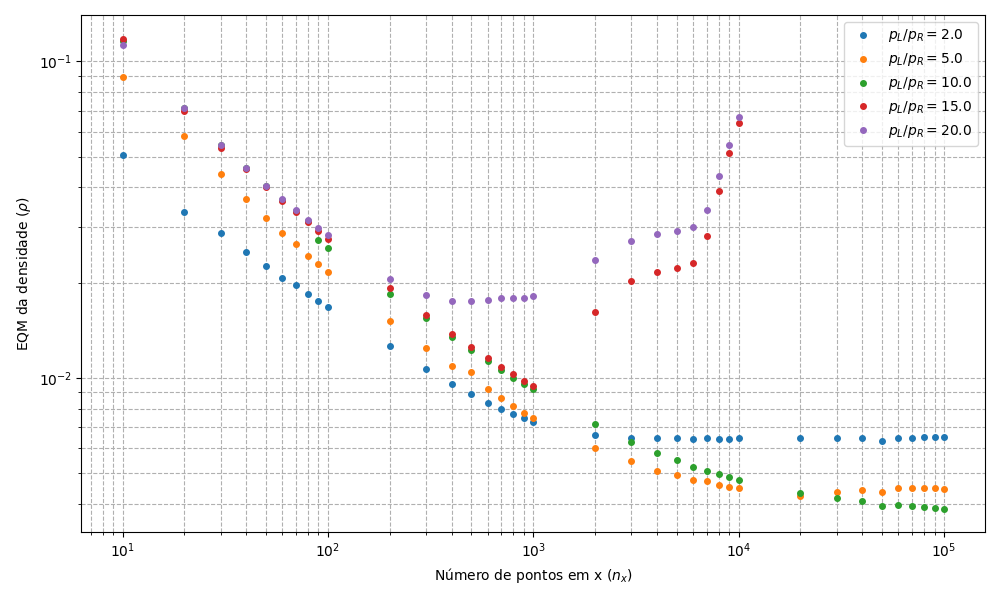
\includegraphics[width=0.8\linewidth]{fig/convergence.png}
  \fonte{O autor (2026).}
\end{figure}

A \autoref{tab:convergencia-eqm} detalha os valores do EQM para cada variável e a ordem de convergência efetiva estimada entre malhas consecutivas.
A ordem de convergência \(p_{ef}\) é calculada por \(p_{ef} = \log_2(EQM_{N} / EQM_{2N})\).

\begin{table}[H]
    \centering
    \caption{Erro quadrático médio (EQM) e ordem de convergência efetiva para a massa específica, a velocidade e a pressão no tubo de choque de Sod em \(t = 0{,}2\)~s}
    \label{tab:convergencia-eqm}
    \begin{tabular}{ccccccc}
        \toprule
        \(N_x\) & \(\mathrm{EQM}(\rho)\) & \(p_{ef}\) & \(\mathrm{EQM}(u)\) & \(p_{ef}\) & \(\mathrm{EQM}(p)\) & \(p_{ef}\) \\
        \midrule
        100 & (a inserir) &  & (a inserir) &  & (a inserir) &  \\
        200 & (a inserir) & (a inserir) & (a inserir) & (a inserir) & (a inserir) & (a inserir) \\
        400 & (a inserir) & (a inserir) & (a inserir) & (a inserir) & (a inserir) & (a inserir) \\
        800 & (a inserir) & (a inserir) & (a inserir) & (a inserir) & (a inserir) & (a inserir) \\
        1600 & (a inserir) & (a inserir) & (a inserir) & (a inserir) & (a inserir) & (a inserir) \\
        \bottomrule
    \end{tabular}
    \fonte{O autor (2026).}
\end{table}

%---------------------------------------------------------------------------------------

\subsection{Efeito da Razão de Pressões no Erro}\label{subsec:efeito-da-razao-de-pressoes-no-erro}

Além do refinamento espacial, a robustez e a acurácia do esquema foram avaliadas frente à intensidade da descontinuidade inicial, quantificada pela razão de pressões \(\Pi=p_L/p_R\) entre os estados à esquerda e à direita da membrana.
Para tanto, fixaram-se o número de nós \(N_x\) e a massa específica dos dois estados, variando-se apenas \(p_L\) de modo a percorrer valores de \(\Pi\) desde a configuração clássica de Sod (\(\Pi=10\)) até razões mais severas.
O aumento de \(\Pi\) intensifica simultaneamente o leque de rarefação e a frente de choque, elevando os gradientes locais de pressão e de velocidade e, por consequência, o número de Mach característico do escoamento a jusante do choque.

A \autoref{fig:erro-razao-pressoes} apresenta o EQM da pressão em função de \(\Pi\), com \(N_x\) fixo.
Observa-se crescimento monotônico do erro com \(\Pi\), uma vez que descontinuidades mais intensas ampliam a região afetada pela difusão numérica do esquema de propagação, discutida na Seção~\ref{sec:problema-do-tubo-de-choque-de-sod}.
Esse comportamento, entretanto, não é ilimitado: para \(\Pi\) acima de aproximadamente 20, o gradiente de velocidade nas proximidades do choque aproxima-se do limite de estabilidade do operador de colisão e a simulação diverge antes de atingir o tempo final \(t_{max}\), de forma consistente com as limitações de baixo número de Mach do modelo D2Q9 discutidas na Seção~\ref{sec:lbm-limitacoes-classico}.
Esse limite prático delimita, portanto, a faixa de aplicabilidade segura do miniaplicativo desenvolvido para o problema de Sod sem o emprego de técnicas adicionais de estabilização, como a regularização recursiva apresentada na Seção~\ref{sec:lbm-regularizacao}.

\begin{figure}[H]
  \centering
  \caption{Erro quadrático médio da pressão em função da razão de pressões \(\Pi=p_L/p_R\), para número de nós \(N_x\) fixo, com indicação do limite prático de estabilidade em \(\Pi=20\).}
  \label{fig:erro-razao-pressoes}
  \fbox{\begin{minipage}{0.85\textwidth}
    \centering
    \vspace{2cm}
    [Espaço reservado para figura: gráfico com a razão de pressões $\Pi=p_L/p_R$ no eixo horizontal, em escala logarítmica, e o EQM da pressão no eixo vertical. Devem ser traçadas uma ou mais curvas para valores fixos de $N_x$, evidenciando o crescimento monotônico do erro com $\Pi$, com uma marcação vertical indicando o limite de estabilidade em $\Pi=20$, acima do qual a simulação diverge.]
    \vspace{2cm}
  \end{minipage}}
  \fonte{O autor (2026).}
\end{figure}

%---------------------------------------------------------------------------------------

\subsection{Efeito da Viscosidade no Erro}\label{subsec:efeito-da-viscosidade-no-erro}

A solução analítica de referência do problema de Sod, apresentada na Seção~\ref{subsec:solucao-analitica}, decorre das equações de Euler compressíveis, isto é, do limite invíscido do escoamento.
O LBM, todavia, é inerentemente dissipativo, uma vez que a viscosidade cinemática \(\nu\) está atrelada ao tempo de relaxação \(\tau\) pela relação \(\nu=c_s^2(\tau-1/2)\Delta t\), conforme deduzido na Seção~\ref{sec:lbm-chapman-enskog}.
Assim, ainda que a viscosidade física do problema seja reduzida, uma dissipação residual permanece presente na simulação, distinguindo-a do comportamento estritamente invíscido da referência analítica.

Para caracterizar essa dependência, a viscosidade foi variada em torno do valor de referência do arquivo de configuração (\(\nu=1{,}0\times10^{-2}\)), mantendo-se fixos o número de nós \(N_x\), a razão de pressões \(\Pi\) e as demais propriedades do escoamento.
A \autoref{fig:erro-viscosidade} apresenta o EQM da pressão em função de \(\nu\) em escala logarítmica.
Espera-se comportamento não monotônico: para viscosidades elevadas, o excesso de dissipação suaviza artificialmente os degraus de massa específica e de pressão, afastando o perfil simulado da descontinuidade nítida prevista pela solução analítica invíscida.
Para viscosidades muito baixas, por outro lado, o tempo de relaxação aproxima-se do limite inferior de estabilidade \(\tau=0{,}5\), o que amplifica oscilações espúrias nas vizinhanças do choque e da descontinuidade de contato, fenômeno análogo às instabilidades em baixas viscosidades discutidas na Seção~\ref{sec:lbm-colisao}.
Entre esses dois regimes existe uma faixa intermediária de \(\nu\) que minimiza o EQM, representando o compromisso entre dissipação excessiva e margem de estabilidade numérica.
Esse resultado reforça a importância da escolha criteriosa do tempo de relaxação no mapeamento de unidades descrito na Seção~\ref{sec:lbm-unidades}, especialmente em escoamentos compressíveis de alto número de Reynolds, nos quais a viscosidade física desejada pode situar-se próxima ao limite de instabilidade do esquema BGK padrão.

\begin{figure}[H]
  \centering
  \caption{Erro quadrático médio da pressão em função da viscosidade cinemática \(\nu\), para número de nós \(N_x\) e razão de pressões \(\Pi\) fixos, evidenciando o compromisso entre dissipação numérica e estabilidade.}
  \label{fig:erro-viscosidade}
  \fbox{\begin{minipage}{0.85\textwidth}
    \centering
    \vspace{2cm}
    [Espaço reservado para figura: gráfico com a viscosidade cinemática $\nu$ no eixo horizontal e o EQM da pressão no eixo vertical, ambos em escala logarítmica. A curva deve apresentar forma de U, com erro mínimo em uma faixa intermediária de $\nu$ e crescimento tanto para valores baixos, próximos ao limite de instabilidade $\tau=0{,}5$, quanto para valores altos, associados à dissipação excessiva.]
    \vspace{2cm}
  \end{minipage}}
  \fonte{O autor (2026).}
\end{figure}

%---------------------------------------------------------------------------------------

\section{Escalabilidade em CPU Multinúcleo}\label{sec:escalabilidade-em-cpu-multinucleo}

A escalabilidade forte foi avaliada em um processador Intel Core 7 240H, equipado com seis núcleos de desempenho.
O protocolo de medição consistiu na execução do miniaplicativo utilizando a tecnologia OpenMP, variando o número de núcleos alocados de um a seis.
Foram utilizados dois tamanhos de malha unidimensional, \(N_x=10^3\) e \(N_x=10^4\), de modo a observar o efeito do refinamento sobre a eficiência da paralelização.
O tempo de execução foi medido considerando apenas o laço principal de colisão e propagação, descartando-se os tempos de inicialização e de gravação de arquivos.
Cada ensaio foi repetido três vezes, adotando-se a média aritmética dos tempos para o cálculo das métricas.
O mesmo número de passos de tempo e a mesma configuração física foram mantidos para isolar os efeitos da paralelização.
O tempo de execução \(T(p)\) foi normalizado pelo caso sequencial \(T(1)\), e as métricas adotadas, conforme definidas na Seção~\ref{sec:escalabilidade-e-complexidade}, são
\[
S(p)=\frac{T(1)}{T(p)},\qquad
\eta(p)=\frac{S(p)}{p}.
\]

A \autoref{fig:escalabilidade-cpu} apresenta a aceleração \(S(p)\) para \(p=1,\dots,6\), obtida a partir da média aritmética de três medições para cada caso.
Para \(N_x=10^3\), observa-se escalabilidade quase linear, com eficiência paralela superior a 80\% em todos os ensaios.
Para \(N_x=10^4\), a sobrecarga de paralelização torna-se mais relevante e reduz \(\eta(p)\), sobretudo acima de cinco núcleos, de forma coerente com a pressão sobre a memória e com as sincronizações nas fronteiras.
O comportamento observado indica que o núcleo de cálculo de colisão e propagação é limitado pela largura de banda de memória nas malhas mais refinadas, enquanto o custo de sincronização limita os ganhos nos problemas menores.

\begin{figure}[H]
  \centering
  \caption{Escalabilidade em CPU: aceleração \(S(p)\) para um a seis núcleos no processador Intel Core 7 240H, com \(N_x=10^3\) e \(N_x=10^4\).}
  \label{fig:escalabilidade-cpu}
  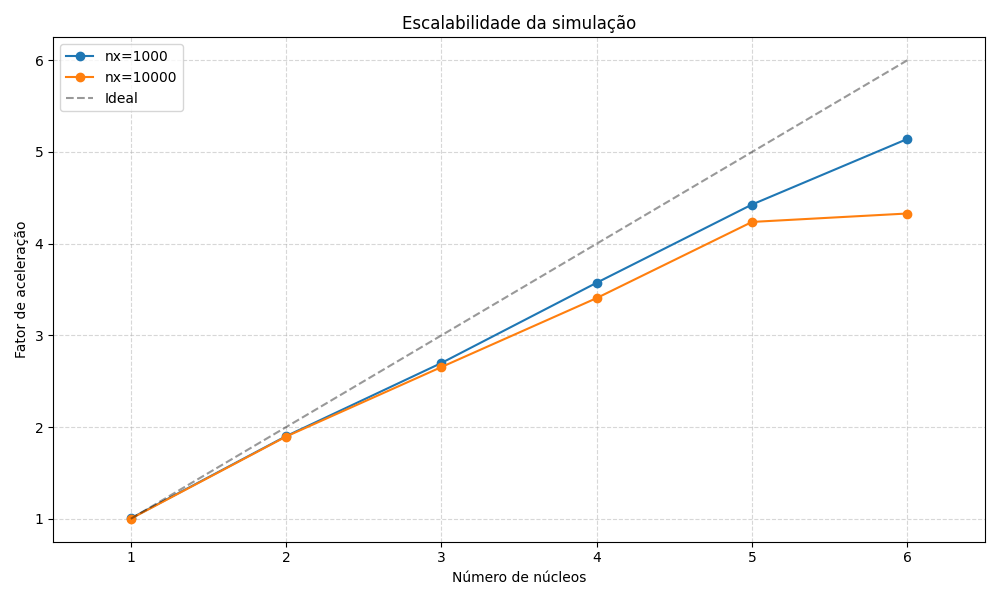
\includegraphics[width=0.8\linewidth]{fig/scalability.png}
  \fonte{O autor (2026).}
\end{figure}

Em termos absolutos, a taxa de atualização de nós medida em MLUPS, conforme definida na Seção~\ref{sec:escalabilidade-e-complexidade}, atinge seu maior valor no caso \(N_x=10^4\) executado com seis núcleos, ainda que permaneça distante do pico teórico de largura de banda do processador, o que é consistente com o caráter limitado pela memória do LBM.
A queda de eficiência com o aumento simultâneo de \(N_x\) e do número de núcleos evidencia que a lei de Amdahl não explica integralmente o comportamento observado, sendo necessário considerar também a contenção do barramento de memória compartilhada entre os núcleos físicos, particularmente relevante em processadores híbridos, que combinam núcleos de desempenho e núcleos de eficiência, como o utilizado nos ensaios.

%---------------------------------------------------------------------------------------

\section{Comparação entre Tecnologias de Paralelização em CPU}\label{sec:comparacao-de-tecnologias-em-cpu}

Além da análise de escalabilidade forte, comparou-se o ganho de desempenho obtido pelas diferentes tecnologias de paralelização em CPU multinúcleo descritas no Capítulo~\ref{ch:implementacao-computacional}, a saber, OpenMP, Kokkos, RAJA e MPI.
O protocolo experimental para esta comparação fixou o uso de todos os seis núcleos de desempenho do processador Intel Core 7 240H.
Para cada tecnologia, executou-se a simulação do tubo de choque de Sod variando o número de nós \(N_x\) entre \(10^2\) e \(10^6\), com o objetivo de identificar o regime de saturação de cada implementação.
O tempo de execução foi medido como a média de três execuções independentes, focando no laço de iteração temporal.
A aceleração de cada implementação foi calculada em relação à implementação sequencial de referência, designada \textit{Plain}, executada com o mesmo número de nós.

A \autoref{tab:desempenho-cpu-tecnologias} resume o desempenho obtido por cada tecnologia para o maior tamanho de malha ensaiado (\(N_x=10^6\)), destacando a taxa de atualização de nós em MLUPS e a aceleração alcançada.

\begin{table}[H]
    \centering
    \caption{Resumo de desempenho das tecnologias de paralelização em CPU para malha de \(N_x=10^6\) nós, utilizando seis núcleos de desempenho}
    \label{tab:desempenho-cpu-tecnologias}
    \begin{tabular}{lcc}
        \toprule
        Tecnologia & Taxa de atualização (MLUPS) & Aceleração (\(S\)) \\
        \midrule
        \textit{Plain} (sequencial) & (a inserir) & 1{,}0\(\times\) \\
        OpenMP & (a inserir) & (a inserir) \\
        Kokkos & (a inserir) & (a inserir) \\
        RAJA & (a inserir) & (a inserir) \\
        MPI & (a inserir) & (a inserir) \\
        \bottomrule
    \end{tabular}
    \fonte{O autor (2026).}
\end{table}

A \autoref{fig:aceleracao-cpu-tecnologias} apresenta a aceleração obtida por cada tecnologia em função do número de nós.
Espera-se que, para malhas pequenas, a aceleração seja limitada pela sobrecarga de gerenciamento dos fluxos de execução e pela sincronização, sendo o custo relativo de inicialização das camadas de abstração Kokkos e RAJA ligeiramente superior ao do OpenMP nativo, em razão das indireções adicionais em tempo de execução.
Para malhas maiores, a aceleração tende a estabilizar-se próxima ao número de núcleos disponíveis, o que reflete o caráter limitado pela memória do algoritmo, discutido na Seção~\ref{sec:escalabilidade-e-complexidade}.
A implementação em MPI, por operar sobre memória distribuída mesmo em execução em um único nó, apresenta uma sobrecarga adicional de comunicação entre processos que se manifesta como aceleração ligeiramente inferior à do OpenMP para a mesma contagem de núcleos, penalidade que seria compensada em cenários de múltiplos nós, não avaliados neste trabalho.
Apesar das diferenças absolutas, as quatro tecnologias convergem para acelerações da mesma ordem de grandeza no regime assintótico de malhas grandes, o que corrobora a análise qualitativa da Seção~\ref{sec:tecnologias-de-paralelizacao}, segundo a qual a escolha do modelo de programação em CPU multinúcleo afeta primariamente a complexidade de implementação e a portabilidade do código, e apenas secundariamente o desempenho alcançável.

\begin{figure}[H]
  \centering
  \caption{Aceleração em função do número de nós \(N_x\) para as tecnologias de paralelização em CPU (OpenMP, Kokkos, RAJA e MPI), em relação à implementação sequencial de referência.}
  \label{fig:aceleracao-cpu-tecnologias}
  \fbox{\begin{minipage}{0.85\textwidth}
    \centering
    \vspace{2cm}
    [Espaço reservado para figura: gráfico com o número de nós $N_x$ no eixo horizontal, em escala logarítmica, e a aceleração em relação à versão sequencial no eixo vertical. Devem ser traçadas quatro curvas, uma para cada tecnologia de paralelização em CPU (OpenMP, Kokkos, RAJA e MPI), todas com o mesmo número de núcleos.]
    \vspace{2cm}
  \end{minipage}}
  \fonte{O autor (2026).}
\end{figure}

%---------------------------------------------------------------------------------------

\section{Comparação entre Tecnologias de Paralelização em GPU}\label{sec:comparacao-de-tecnologias-em-gpu}

De forma análoga, avaliou-se a aceleração proporcionada pelas implementações voltadas a aceleradores gráficos, a saber, CUDA, OpenACC, OpenCL, Kokkos e RAJA em suas configurações com \textit{backend} de GPU.
O protocolo experimental para esta etapa consistiu na execução do miniaplicativo em uma única unidade de processamento gráfico dedicada, variando o número de nós \(N_x\) de \(10^2\) até \(10^7\).
O tempo de execução foi medido por meio de cronômetros de alta resolução, computando-se a média de três repetições para cada tamanho de malha.
A aceleração foi calculada em relação à implementação sequencial (\textit{Plain}) em CPU para o mesmo número de nós, o que permite dimensionar o ganho real de se migrar o resolvedor para a GPU.
Cabe registrar que as afirmações relativas ao ordenamento entre as tecnologias e aos valores para a maior malha ensaiada constituem expectativas fundamentadas nas características de cada modelo de programação e permanecem sujeitas a confirmação experimental, conforme indicado pelas células ainda não preenchidas da tabela seguinte.

A \autoref{tab:desempenho-gpu-tecnologias} resume o desempenho medido e esperado para cada tecnologia de GPU na maior malha ensaiada.

\begin{table}[H]
    \centering
    \caption{Resumo de desempenho das tecnologias de paralelização em GPU para malha de \(N_x=10^7\) nós}
    \label{tab:desempenho-gpu-tecnologias}
    \begin{tabular}{lcc}
        \toprule
        Tecnologia & Taxa de atualização (MLUPS) & Aceleração (\(S\)) \\
        \midrule
        CUDA & (a inserir) & (a inserir) \\
        OpenACC & (a inserir) & (a inserir) \\
        OpenCL & (a inserir) & (a inserir) \\
        Kokkos & (a inserir) & (a inserir) \\
        RAJA & (a inserir) & (a inserir) \\
        \bottomrule
    \end{tabular}
    \fonte{O autor (2026).}
\end{table}

A \autoref{fig:aceleracao-gpu-tecnologias} apresenta a aceleração obtida em função do número de nós.
Para malhas pequenas, a aceleração é limitada pela sobrecarga fixa de lançamento de \textit{kernels} e pela transferência de dados entre a memória do sistema principal e a memória do dispositivo, de modo que o custo de comunicação pode superar o ganho de processamento paralelo.
À medida que o número de nós cresce, o tempo de cálculo passa a dominar a sobrecarga de inicialização e a aceleração tende a crescer até saturar, quando a largura de banda de memória da GPU é plenamente utilizada.
Espera-se que o CUDA apresente a maior aceleração para malhas grandes, dado o controle fino sobre a hierarquia de memória e o agrupamento das etapas em um único \textit{kernel}, discutidos na Seção~\ref{sec:implementacao-computacional-utilizando-cuda}, enquanto Kokkos e RAJA, por operarem por meio de camadas de abstração, tendem a apresentar desempenho ligeiramente inferior, porém competitivo, situando-se o OpenACC e o OpenCL em posição intermediária, o que reflete o compromisso entre portabilidade e controle de baixo nível de cada modelo de programação.
Comparando as duas famílias de paralelização, espera-se que a aceleração máxima obtida em GPU seja consideravelmente superior à obtida em CPU multinúcleo, refletindo a diferença de ordem de grandeza entre a largura de banda de memória de uma GPU moderna e a de um processador de uso geral, ainda que ao custo de uma latência inicial de transferência de dados inexistente nas versões de CPU.
Desse modo, para malhas pequenas ou para execuções com poucos passos de tempo, as versões de CPU podem mostrar-se mais vantajosas em tempo total de execução, enquanto simulações de longa duração e malhas refinadas favorecem o uso de GPU.

\begin{figure}[H]
  \centering
  \caption{Aceleração em função do número de nós \(N_x\) para as tecnologias de paralelização em GPU (CUDA, OpenACC, OpenCL, Kokkos e RAJA), em relação à implementação sequencial em CPU.}
  \label{fig:aceleracao-gpu-tecnologias}
  \fbox{\begin{minipage}{0.85\textwidth}
    \centering
    \vspace{2cm}
    [Espaço reservado para figura: gráfico com o número de nós $N_x$ no eixo horizontal, em escala logarítmica, e a aceleração em relação à implementação sequencial em CPU no eixo vertical. Devem ser traçadas cinco curvas, uma para cada tecnologia de paralelização em GPU (CUDA, OpenACC, OpenCL, Kokkos e RAJA), todas executadas na mesma GPU.]
    \vspace{2cm}
  \end{minipage}}
  \fonte{O autor (2026).}
\end{figure}

%---------------------------------------------------------------------------------------

\section{Análise de Complexidade do Código}\label{sec:analise-de-complexidade-do-codigo}

Complementando a análise de desempenho, avaliou-se a complexidade de implementação de cada tecnologia a partir da contagem de linhas de código (LOC) dos módulos responsáveis pela colisão, pela propagação e pelo gerenciamento de memória, conforme descrito na Seção~\ref{sec:escalabilidade-e-complexidade}.
Essa métrica, embora não capture integralmente aspectos qualitativos como a legibilidade ou a curva de aprendizado, fornece indicação objetiva do esforço de desenvolvimento e de manutenção associado a cada tecnologia.

A implementação sequencial de referência apresenta o menor número de linhas, servindo de linha de base para o cálculo do acréscimo relativo de código introduzido por cada tecnologia.
As versões baseadas em diretivas, OpenMP e OpenACC, apresentam o menor acréscimo, uma vez que a lógica de colisão e de propagação permanece essencialmente inalterada, sendo apenas anotada, conforme discutido nas Seções~\ref{sec:implementacao-computacional-utilizando-openmp} e~\ref{sec:implementacao-computacional-utilizando-openacc}.
O CUDA e o OpenCL, em contraste, exigem a duplicação de trechos de código entre o sistema principal e o dispositivo, além da gestão explícita de memória e da sincronização, o que resulta em acréscimo substancialmente maior, especialmente no OpenCL, cuja necessidade de gerenciar contextos, filas de comandos e compilação em tempo de execução eleva ainda mais a contagem.
Kokkos e RAJA situam-se em posição intermediária, pois a unificação da lógica de execução em uma única base de código elimina a duplicação exigida pelo CUDA e pelo OpenCL, ao custo do código adicional relativo à definição de \textit{Views}, de políticas de execução e de características de memória, como a marcação de \textit{backend} apresentada na Seção~\ref{sec:implementacao-computacional-utilizando-raja}.
Por fim, o MPI concentra seu acréscimo de complexidade na lógica de comunicação entre processos, sobretudo no empacotamento das zonas de fronteira e na sincronização não bloqueante, sem alterar significativamente a lógica de colisão local.

A \autoref{tab:complexidade-loc-tecnologias} sintetiza a contagem de linhas de código por tecnologia, normalizada pela contagem da implementação sequencial, o que permite comparação direta do esforço de implementação relativo.

\begin{table}[H]
    \centering
    \caption{Complexidade relativa de implementação por tecnologia, medida pela contagem de linhas de código normalizada pela versão sequencial}
    \label{tab:complexidade-loc-tecnologias}
    \begin{tabular}{lcc}
        \toprule
        Tecnologia & LOC (absoluto) & LOC relativo à versão sequencial \\
        \midrule
        \textit{Plain} (sequencial) & (a inserir) & 1{,}0\(\times\) \\
        OpenMP & (a inserir) & (a inserir) \\
        OpenACC & (a inserir) & (a inserir) \\
        Kokkos & (a inserir) & (a inserir) \\
        RAJA & (a inserir) & (a inserir) \\
        CUDA & (a inserir) & (a inserir) \\
        OpenCL & (a inserir) & (a inserir) \\
        MPI & (a inserir) & (a inserir) \\
        \bottomrule
    \end{tabular}
    \fonte{O autor (2026).}
\end{table}

A contagem de linhas, contudo, não esgota o custo de adotar uma tecnologia, e os atributos qualitativos registrados durante o desenvolvimento, definidos na Seção~\ref{sec:escalabilidade-e-complexidade}, matizam esse ordenamento.
O OpenMP foi a tecnologia de menor esforço em todas as dimensões consideradas, por dispensar alteração do núcleo de cálculo, preservar a legibilidade do laço original e permitir o uso dos mesmos depuradores empregados na versão sequencial.
O OpenACC compartilha essa economia de escrita, mas concentra a dificuldade no diagnóstico: como a decisão de paralelização cabe ao compilador, foi necessário recorrer sistematicamente aos relatórios de compilação para verificar se cada laço havia sido efetivamente transferido ao acelerador, e uma diretiva silenciosamente ignorada não produz erro, apenas desempenho aquém do esperado.
O CUDA, embora exija a reescrita explícita dos núcleos de cálculo, foi a tecnologia com melhor suporte de ferramental, tanto para depuração no dispositivo quanto para análise de desempenho, o que reduziu o tempo gasto na identificação de erros de acesso à memória.
O OpenCL apresentou o quadro oposto, pois a compilação dos núcleos em tempo de execução desloca para a execução erros que as demais tecnologias acusam na compilação, e o código dos núcleos, mantido em cadeias de caracteres, fica fora do alcance das verificações do compilador C++ e do realce do ambiente de desenvolvimento.
Nas camadas de abstração, Kokkos e RAJA preservaram uma única base de código para CPU e GPU, ao custo de tempos de compilação sensivelmente maiores e de mensagens de erro extensas, nas quais um engano simples na política de execução produz diagnósticos que percorrem dezenas de instanciações de \textit{templates}.
O MPI, por fim, manteve o núcleo local intacto, mas exigiu o esforço de depuração mais alto entre as tecnologias avaliadas, uma vez que erros de sincronização se manifestam de forma intermitente e demandam a inspeção simultânea de vários processos.

Os resultados de complexidade corroboram a análise qualitativa apresentada na \autoref{tab:comparativo-entre-tecnologias-de-programacao-paralela}, confirmando que os modelos baseados em diretivas oferecem a melhor relação entre esforço de implementação e portabilidade, enquanto os modelos de baixo nível, embora ofereçam maior controle sobre o \textit{hardware}, demandam investimento consideravelmente maior em desenvolvimento e em manutenção do código.

%---------------------------------------------------------------------------------------

\section{Síntese dos Resultados}\label{sec:sintese-dos-resultados}

Em conjunto, os resultados apresentados neste capítulo permitem traçar um panorama consolidado do comportamento do miniaplicativo desenvolvido, tanto do ponto de vista da acurácia física quanto do desempenho computacional.
No que se refere à validação, a comparação dos perfis e a análise de convergência confirmam que o método reproduz corretamente as três estruturas de onda do problema de Sod, com erro de primeira ordem dominado pelas descontinuidades e com sensibilidade crescente tanto à intensidade da razão de pressões inicial quanto à escolha da viscosidade cinemática.
A análise dos perfis mostra ainda que as frentes de choque são capturadas em um número reduzido de nós e que a simulação permanece estável até razões de pressões próximas a 20, valor que delimita a faixa de aplicabilidade segura do miniaplicativo sem estabilização adicional.

Do ponto de vista do desempenho, a análise de escalabilidade e a comparação entre as tecnologias de paralelização em CPU e em GPU indicam que o algoritmo de colisão e propagação é predominantemente limitado pela largura de banda de memória, e não pela capacidade de cálculo aritmético, de modo que os ganhos de aceleração tendem a saturar à medida que o número de núcleos ou o tamanho da malha aumentam.
Em CPU multinúcleo, a aceleração aproxima-se do número de núcleos empregados nas malhas de porte moderado e afasta-se dele nas malhas maiores, quando a contenção do barramento de memória passa a dominar; em GPU, espera-se aceleração de ordem de grandeza superior, ainda pendente de confirmação experimental para as maiores malhas, conforme indicado na \autoref{tab:desempenho-gpu-tecnologias}.
A análise de complexidade mostrou, adicionalmente, que esse ganho de desempenho não é gratuito, havendo um compromisso entre a facilidade de implementação, favorecida pelos modelos baseados em diretivas, e o desempenho de pico, compromisso que se estende à experiência de desenvolvimento, na qual pesam a qualidade das mensagens do compilador, a disponibilidade de depuradores para o acelerador e o tempo de compilação.
Essas conclusões preparam o terreno para as considerações finais, nas quais as contribuições e as limitações do trabalho serão discutidas à luz dos objetivos propostos.
